
\Chapter{Tervezés}

Itt kezdődik a dolgozat lényegi része, úgy értve, hogy a saját munka bemutatása.
Jellemzően ebben szerepelni szoktak blokkdiagramok, a program struktúrájával foglalkozó leírások.
Ehhez célszerű UML ábrákat (például osztály- és szekvenciadiagramokat) használni.

Amennyiben a dolgozat inkább kutatás jellegű, úgy itt lehet konkretizálni a kutatási módszertant, a kutatás tervezett lépéseit, az indoklást, hogy mit, miért és miért pont úgy érdemes csinálni, ahogyan az a későbbiekben majd részletezésre kerül.

Ebben a fejezetben az implementáció nem kell, hogy túl nagy szerepet kapjon.
Ez még csak a tervezési fázis.
(Nyilván ha olyan a téma, hogy magának az implementációnak a módjával foglalkozik, adott formális nyelvet mutat be, úgy a kódpéldákat már innen sem lehet kihagyni.)

\Section{Követelmények}

\subsection{Általános leírás}
Egy olyan elosztott rendszer környezetben működő szoftver létrehozása a cél, ami képes a drónszállítás közben keletkező valóságnak megfelelő adatokat szimulálni és hatékonyan feldolgozni.
Ezeknek az adatoknak a feldolgozását vizsgálom, több kontextusból.
Egyrészt a hálózaton való kommunikaáció hatékonyságát vizsgálom, tehát hogy mennyi adatforgalommal jár a kommunikáció,
és milyen hatékony ennek a kommunikációnak a feldolgozása, azaz a hálózaton használt formátum átalakítása a programban használt formátumra. Másrészt összehasonlítjuk az adatbázisba való mentés hatékonyságát.
Mivel elosztott rendszerekről van szó, nem egy darab program lesz.
Mikro-szervízként működnek majd a programok.
Ez azt jelenti, hogy ha 100 adat feldolgozást végző program fut egy terhelést elosztó proxy mögött, akkor ugyanolyan viselkedés várható mint ha csak 1 program futna.
A drón szenzorai által gyűjtött adatokat telemetria adatoknak nevezzük. A programok egy részének ezeket az adatokat kell tudnia generálni, egy másik részének feldolgoznia.

\subsection{Hatékonyság}
A hatékonyság alatt egyszerre értjük a teljesítményt, tehát hogy mennyire gyors a feldolgozás, és azt is hogy ez a feldolgozás mennyi erőforrást használ.
Célunk hogy a lehető legkevesebb adatforgalommal, a minimális CPU és memóriahasználattal de minél gyorsabban dolgozzuk fel az adatokat.


\subsection{Funkcionális követelmények}
A szimulációban több féle protokolt és adattovábbításra képes formátumot hasonlítunk össze, így a programot úgy kell felépíteni, hogy ki lehessen cserélni ezeket a végpontokat anélkül hogy a program üzleti logikájának működését befolyásolnánk.
Az adatközpontok és drónok közötti telemetria adat kommunikációt és annak feldolgozását összehasonlítjuk egy HTTP 1.1 -en műkodő JSON adatformátumot használó REST~\cite{Wikipedia-REST} API-n, egy HTTP 2 -n futó gRPC-t használó végponton is.
Az adatok mentését is több adatbázison kell tesztelni, így az adatbázisnak is cserélhetőnek kell lennie.

%TODO: ide még írni

\Section{Program struktúra}
\subsection{Architektúra, program felépítés}\label{subsec:architektúra-program-felépítés}
A probléma szimulációja 2 programból~\ref{fig:3program} áll. Egy program az adatközpont, egy program a drónok szerepét veszi fel, és van még egy egyszerű kliens ami,
paraméterek alapján konfigurálja a 2 program működését.
Az két program mikroszervízes struktúrában használhatónak kell lennie, hogy a valódi elosztott rendszeres működést megfelelően tudjuk tesztelni.\\
Az adatközpontot szimuláló program lesz a legbonyolultabb.
Ennek a programnak tudnia kell hibamentesen, adatvesztés nélkül feldolgozni és tárolnia az adatokat amiket a drónok küldenek, és vezérelni kell tudni a drónok indítását, logisztikai feladatait.

\begin{figure}[h]
    \centering
    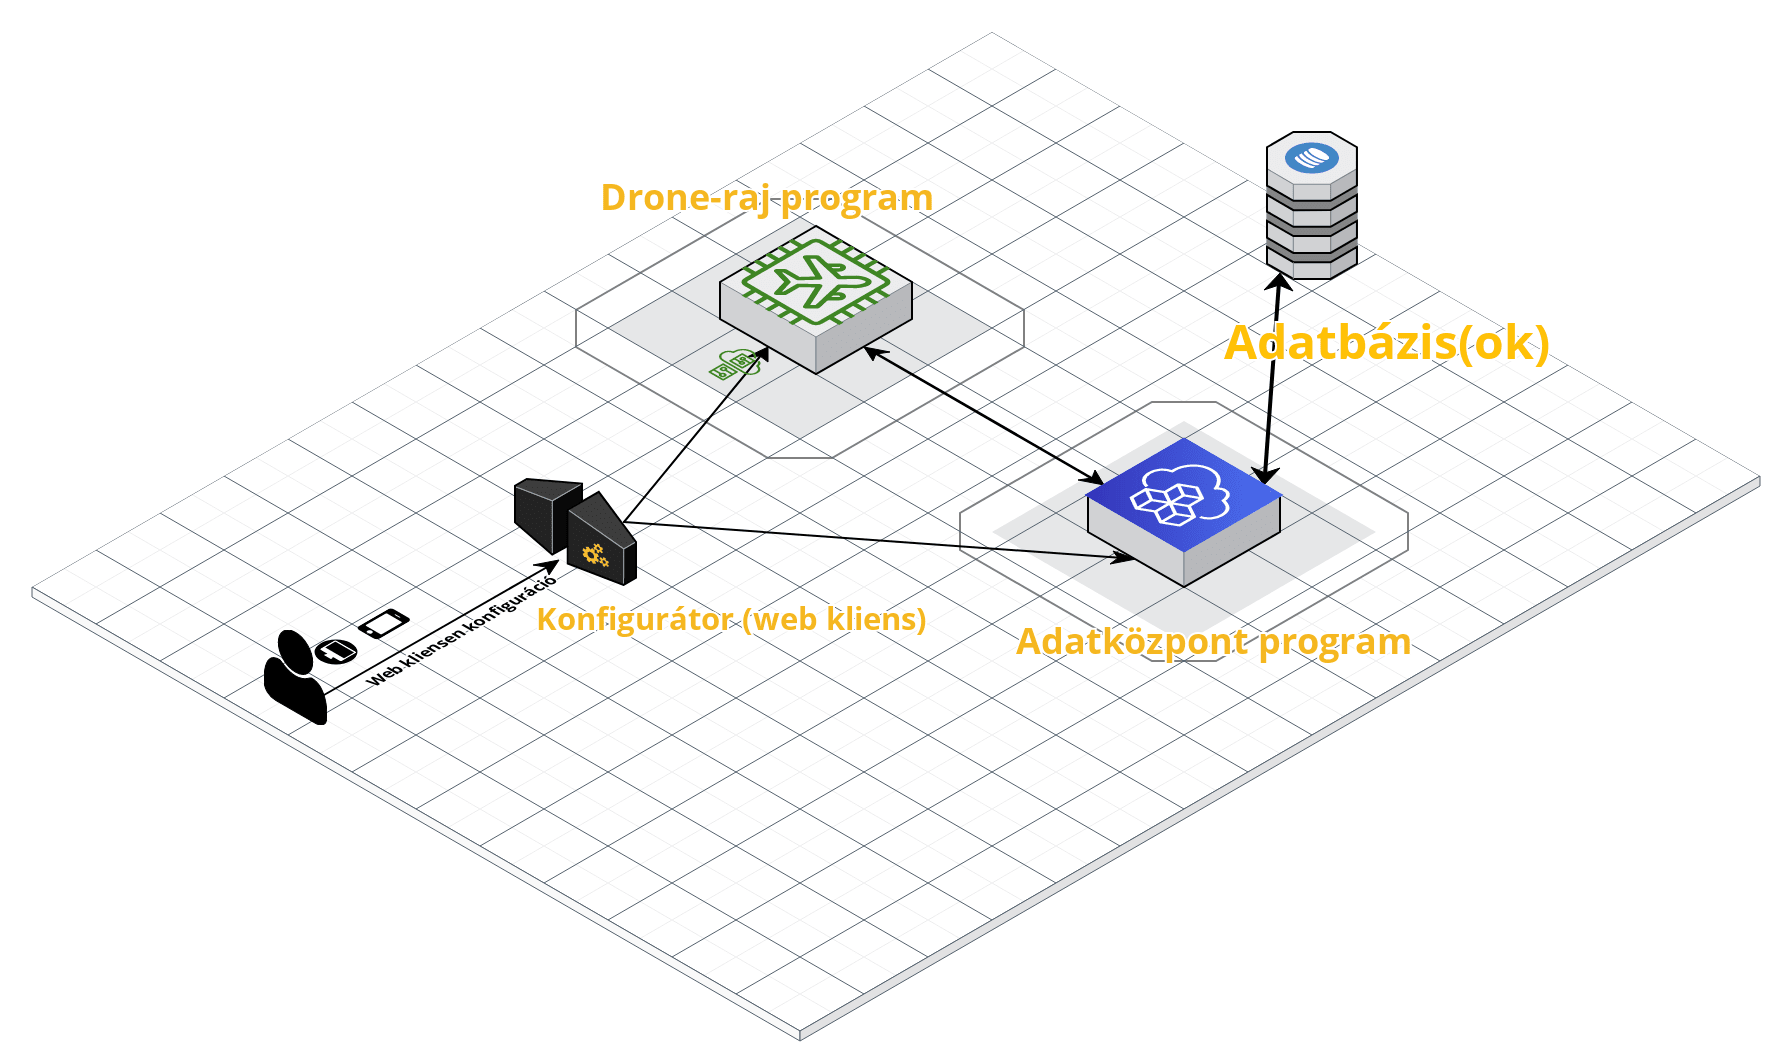
\includegraphics[scale=0.22]{images/szakdolgozat-3-program-abra.png}
    \caption{A 3 program}
    \label{fig:3program}
\end{figure}
Ahhoz hogy a programot a követelmányben megfogalmazott módon építsük fel, értem ez alatt azt hogy több protokollt és adatbázist hasonlítsunk össze egy olyan program architektúrát, felépítést kell választani ami megendegi ezt.
Erre a problémára megoldásként a Hexagonal architektúrát~\ref{fig:hexagonal-inward} és DDD tervezési alapelvet fogom alkalmazni.
\begin{figure}[h]
    \centering
    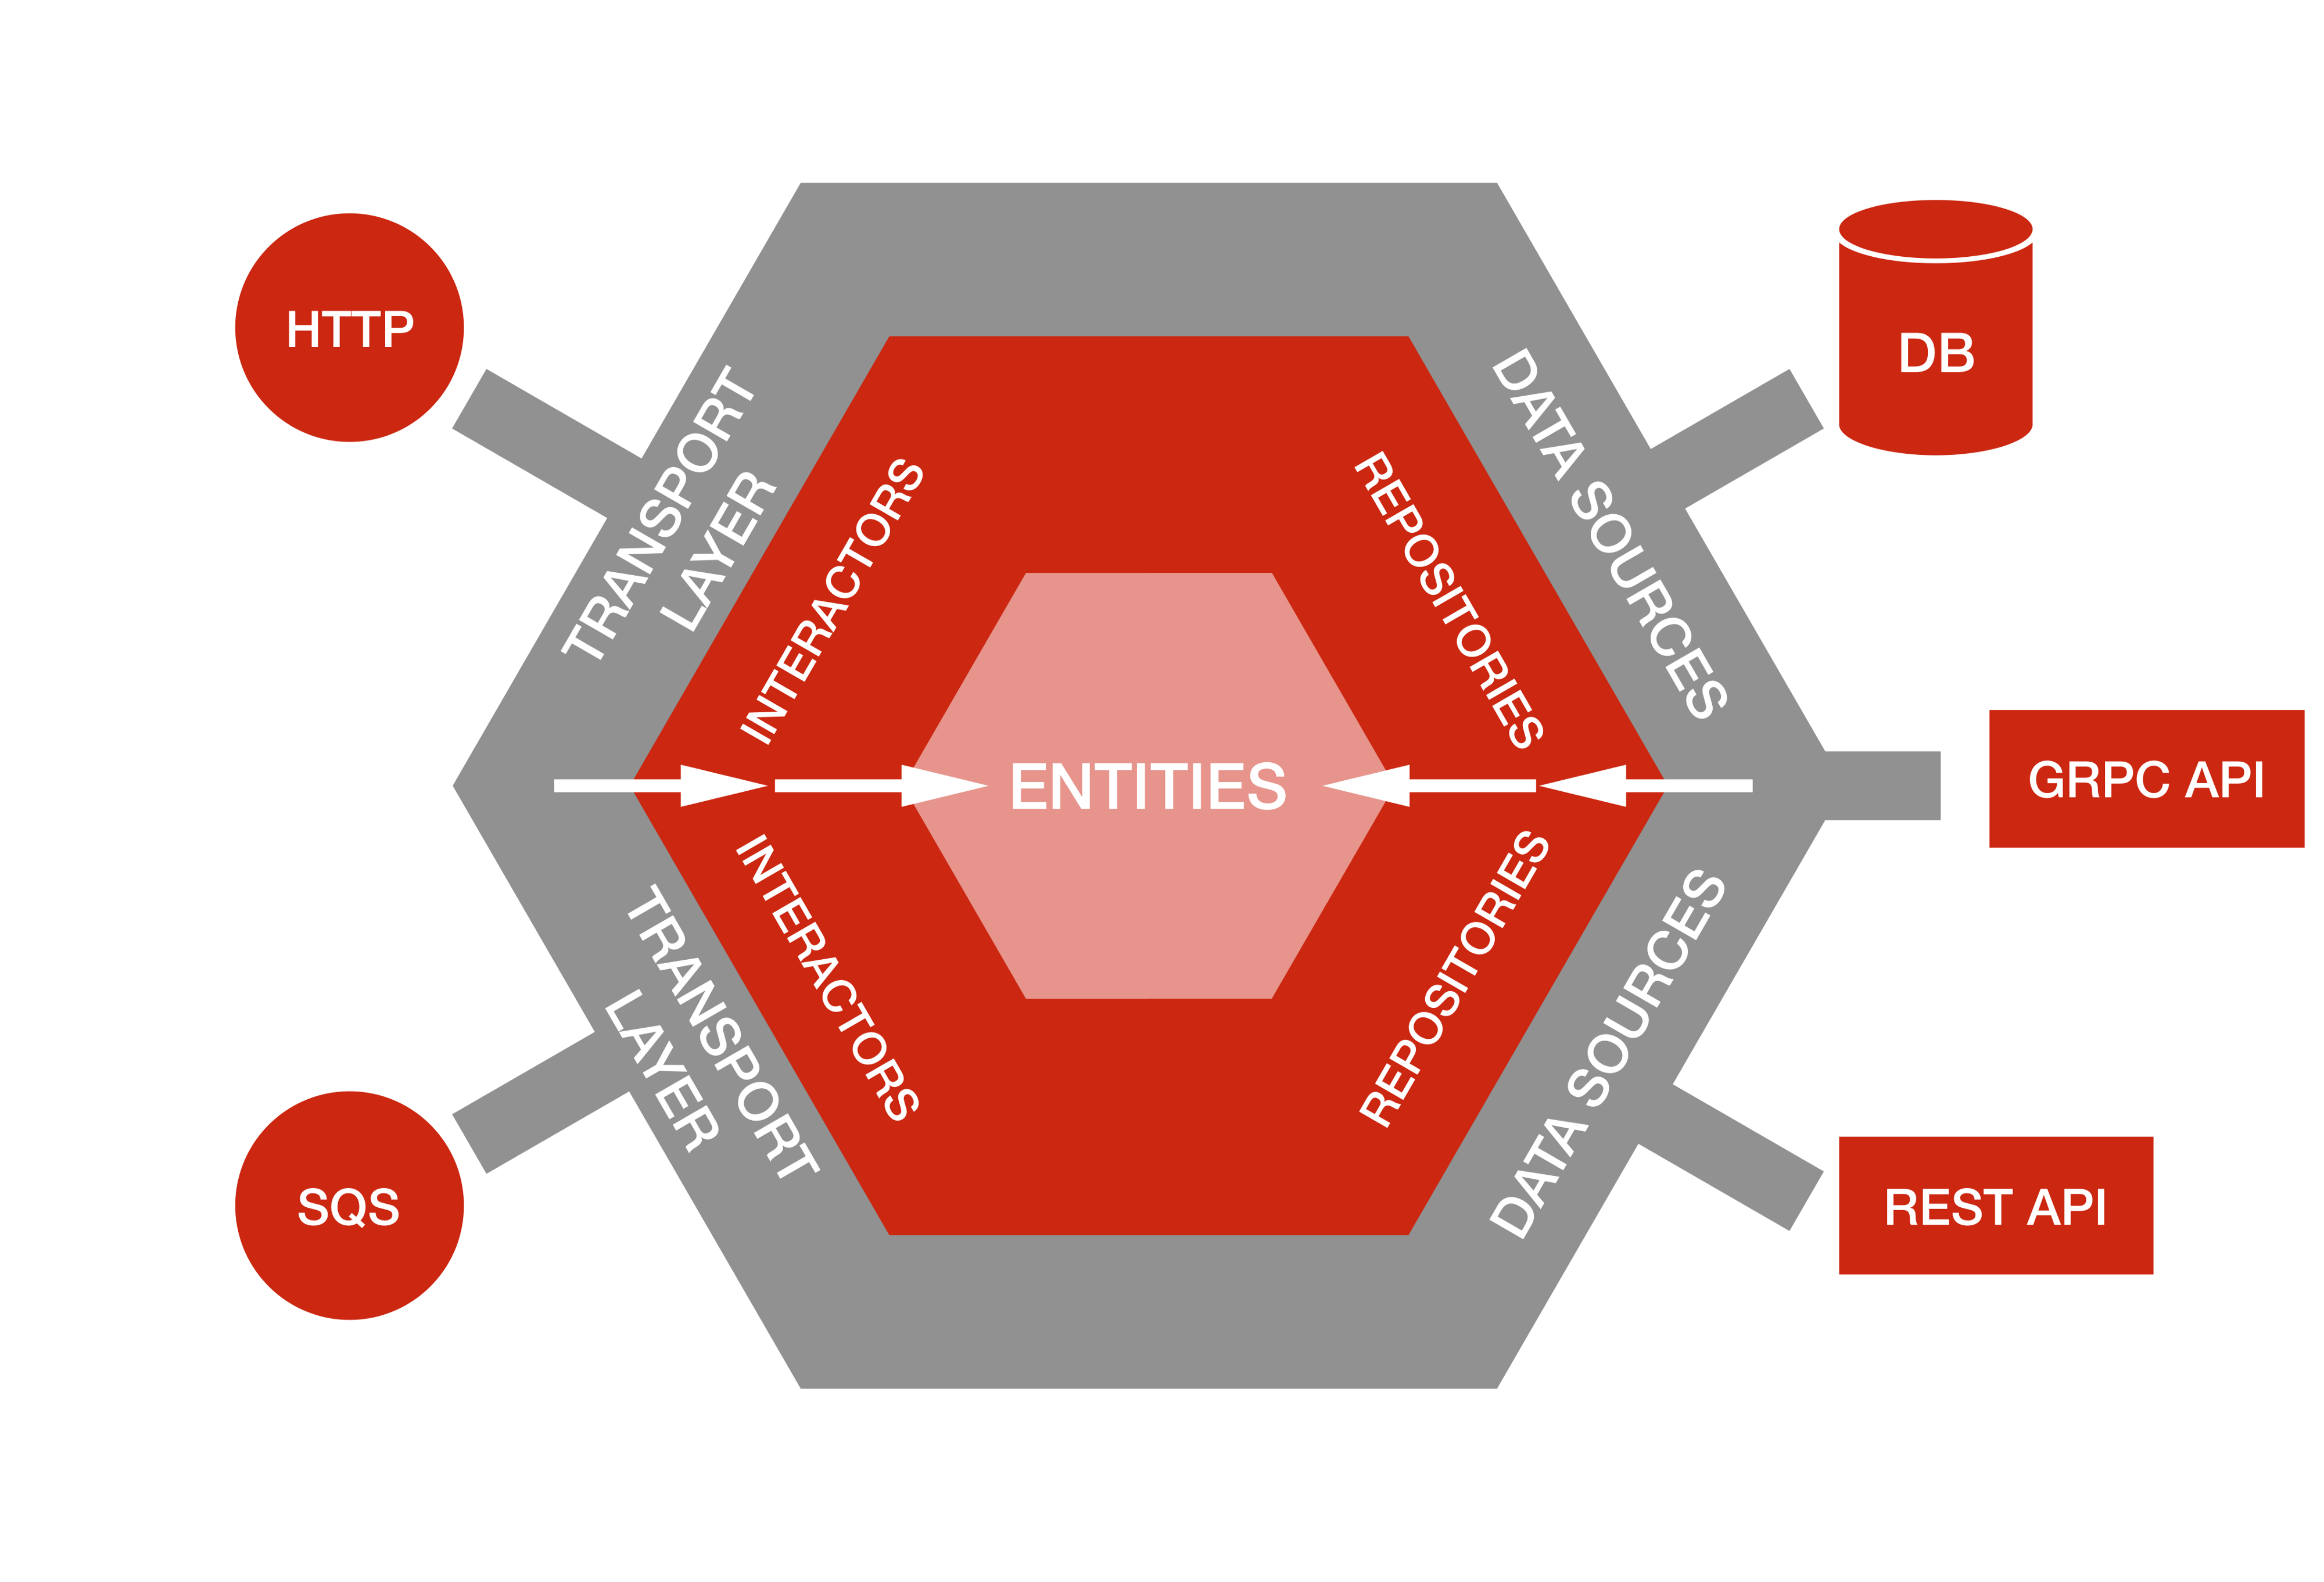
\includegraphics[scale=0.07]{images/hexa-inward.png}
    \caption{Hexagonal architecture inward pointing dependencies}
    \label{fig:hexagonal-inward}
\end{figure}
Így a program belülről kifelé rétegesen epül fel, interfaceket alkalmazva, úgy hogy a pontos implemetáció absztraktálva van, azaz csak az üzleti logikát ismerjük biztosan, minden ráépülő réteg implementációja cserélhető marad.
Minden réteg csak befelé mutat \ref{fig:hexagonal-inward}, így az üzleti logikánk megmaradhat, miközben az alkalmazás teljes infrastuktúráját kicserélhetnénk.
Így a végpontok ha teljesítik az interface elvárásait, csak dependency injection-el kicseréljük a végpontot és minden ugyanúgy működik, ám teljesen más az implementáció.
Azt hogy több fajta input és output végpontot hogy  támogatja az alkalmazás a következő ábra \ref{fig:hexagonal-inward} tökéletesen bemutatja.
Az alkalmazást fel lehet osztani verérlő és vezérelt részre. Ez nagyon jól igazodik az üzleti logikához, egy inputra szinte mindig valamiféle vezérlést várunk el,
tehát ahogz az alkalmazásunkat használjuk, vezéreljük akkor az adatok hatására valamit csináljon. Ezután az alkalmazásunk beszélhet más, külső forrásokkal, amiket az alkalmazás használ, azaz vezéreli őket.
Ilyen lehet egy adatbázis implementációja, vagy egy üzenet sor, amibe adatokat rakunk be, hogy valami más később kiolvassa.
Azért jó ez a felépítés, mert így például mindegy hogy a terminálból valamilyen konzolos applikáción keresztül hívjuk meg az alkalmazásunkat,
vagy egy webes felületről. A vezérelt egységeket is ki lehet cserélni, nem vagyunk röghöz kötve mert egyszer így lett megírva az alkalmazésunk, csak a megfelelő réteget kicseréljük, feltéve hogy megírtuk hozzá az implementációnkat és az implementációnk
az intefészen keresztül teljesít minden feltételt. Így például könnyen átállhatunk relációs adatbázisról egy dokumentum alapúra, vagy egy API-t is kicserélhetünk például JSON REST API-t gRPC-re ha valami miatt szükség van rá.
A Netflix is ezt az architektúrát használja \cite{netflix}, ugyanis a gyors növekedésük közben több skálázhatósággal összefüggő problémába ütköztek, amit úgy oldottak meg hogy
ebben az architektúrában\ref{fig:hexagonal-actor} szétosztották a feladatokat több, az adott kis feladatra megfelelő adatbázisra, mikroszervízre.
\begin{figure}[h]
    \centering
    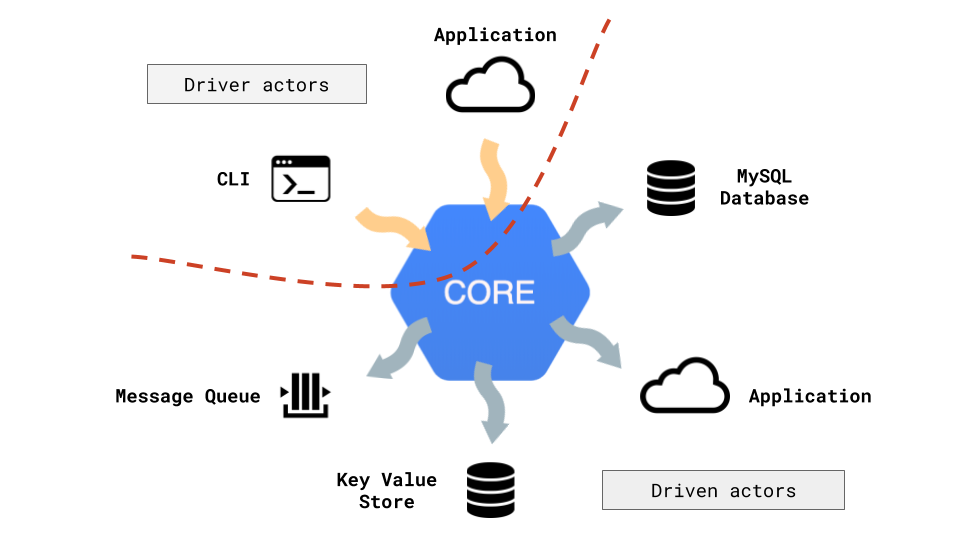
\includegraphics[scale=0.3]{images/hexa-actor.png}
    \caption{Hexagonal architecture ports and adapters}
    \label{fig:hexagonal-actor}
\end{figure}

\subsection{A Hexagonal architektúráról bővebben}\label{subsec:a-hexagonal-architektúráról-bővebben}
A hexagonal architektúra~\cite{hexagonal}, vagy másnéven portok és adapterek architektúra a szoftver tervezés során használt design.
Célja lazán összekapcsolt alkalmazás komponensek létrehozása, amelyek portok és adapterek segítségével könnyen összekapcsolhatóak.
Ez cserélhetővé teszi a program komponenseket bármilyen szinten, és megkönnyíti a teszteket.

Minden komponens nyitott egy "porton".
A komponensek közti kommunikáció ezeken a portokon történik egy adott protokoll alapján.
Ezt a protokollt a célnak megfelelően választjuk meg.
A portok és protokollok egy absztrak API-t definiálnak ami a megfelelő eszközzel implementálható\cite{hexagonal}.
A implementációt az adapterek valósítják meg, az objektum orientált nyelvekben interfész metódusokkal vannak összekötve a program magjával.
Ilyen lehet egy RPC hívás, webes szervíz, REST API, SQL lekérdezés.

\begin{figure}[h]
    \centering
    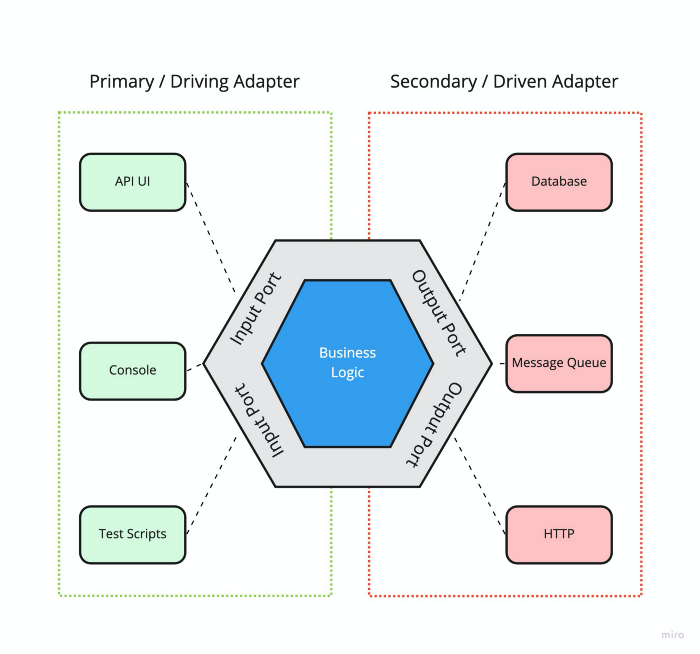
\includegraphics[scale=0.3]{images/ports-adapters}
    \caption{Hexagonal architecture driver and driven actors}
    \label{fig:hexagonal-ports-adapters}
\end{figure}

\subsection{REST architektúra}\label{subsec:rest-architektúra}

A REST (Representational State Transfer) \cite{Wikipedia-REST} egy szoftverarchitektúra típus internet alapú rendszerek számára.
Egy REST architektúrának meg kell felelni a következő megszorításoknak:
\begin{itemize}
    \item Kliens-szerver architektúra
    \item Állapotmentesség
    \item Gyorsítótárazhatóság
    \item Réteges felépítés
    \item Egységes interfész
\end{itemize}

\subsubsection{Kliens-szerver architektúra}
A kliensek el vannak különítve a szerverektől egy egységes interfész által. Az érdekeltségek ilyen nemű szétválasztása azt jelenti, például, hogy a kliensek nem foglalkoznak adattárolással, ami a szerver belső ügye marad, és így a kliens kód hordozhatósága megnő. A szerverek nem foglalkoznak a felhasználói felülettel vagy a kliens állapotával, így a szerverek egyszerűbbek és még skálázhatóbbak lehetnek. A szerverek és kliensek áthelyezhetőek és fejleszthetőek külön-külön is, egészen addig amíg az interfész nem változik meg.
\subsubsection{Állapotmentesség}
A kliens-szerver kommunikáció tovább korlátozott az által, hogy a szerveren nem tárolják a kliens állapotát a kérések között. Minden egyes kérés bármelyik klienstől tartalmazza az összes szükséges információt a kérés kiszolgálásához, és minden állapotot a kliens tárol. A szerver lehet állapottartó; ez a korlátozás csupán azt követeli meg, hogy a szerver oldali erőforrás-állapotok URL által címezhetőek legyenek. Ez nem csak a szerver felügyeletét teszi lehetővé, de megbízhatóbbá teszi őket a hálózati meghibásodásokkal szemben, valamint tovább fokozza a skálázhatóságot.
\subsubsection{Gyorsítótárazhatóság}
Mint ahogy a világhálón, a kliensek itt is képesek gyorsító-tárazni a válaszokat. A válaszoknak ezért impliciten vagy expliciten tartalmazniuk kell, hogy gyorsítótárazhatóak-e vagy sem. Így elkerülhető, hogy a kliens téves vagy elavult adatokat használjon fel újra. Egy jól menedzselt gyorsítótár lehetővé teszi, hogy teljesen megkerüljünk egyes kliens-szerver interakciókat, továbbá megnöveli a rendszer skálázhatóságát és a teljesítményét.
\subsubsection{Réteges felépítés}
Egy kliens általában nem tudja megmondani, hogy direkt csatlakozott-e a végpont szerverhez, vagy közvetítő segítségével. A közvetítő szerverek megnövelhetik a rendszer skálázhatóságát terheléseloszlás kiegyenlítéssel és megosztott gyorsítótárak használatával.
\subsubsection{Egységes interfész}
Az egységes interfész kliens és szerver között egyszerűsíti és kettéválasztja az architektúrát, és lehetővé teszi, hogy egymástól függetlenül fejlődjenek az egyes részek. Az interfész négy irányadó elve alább kerül részletezésre.


Ha ezeket a megkötéseket teljesíti a webes szolgáltatásunk, azt mondhatjuk hogy "RESTful".


\subsubsection{A REST működése}
A kliensek kéréseket indítanak a szerverek felé, a szerverek pedig feldolgozzák a kéréseket és egy választ küldenek vissza.
A kérések és a válaszok erőforrás reprezentációk köré épülnek.
Ezek az erőforrás reprezentációk a mi esetünkben JSON dokumentumok.
Az erőforrásokat az URL címével és a HTTP metódussal azonosítjuk.
A következő példában láthatjuk ahogy egy PUT metódussal és az URL-ben megadott paraméterrel pontosan tudjuk azonosítani mit szeretnénk.
A PUT requestet akkor használjuk ha egy már meglévő erőforrást szeretnénk felülírni, esetünkben az adatbázis konfigurációt kicseréljük.
A :name paraméter pedig megnevezi az erőforrást amire a meglévőt ki szeretnénk cserélni.
Válaszként egy JSON dokumentumot küldünk vissza válaszként a megfelelő státuszkóddal, hogy a kérés sikeres volt vagy sem.

\begin{python}
    router.PUT("/configure/database/:name", func(c echo.Context) error {
        switch c.Param("name") {
            case "mongodb":
            t.ChangeService(m)
            d.ChangeService(m)
            case "postgres":
            t.ChangeService(p)
            d.ChangeService(p)
            default:
            return echo.NewHTTPError(
            http.StatusBadRequest,
            "no such database supported"
            )
        }
        return c.JSON(http.StatusOK, "configuration complete")
    })
\end{python}


\subsection{HTTP/2 gRPC összehasonlítása HTTP/1.1 JSON üzenetváltással}

\paragraph{REST és HTTP 1.1, JSON üzenetváltás}
A mikroszevízes infrastuktúra egy nagyon elterjedt módja az elosztott rendszerek tervezésének.
Sok mikroszervíz a mai napig REST API-n kommunikál, HTTP 1.1-es protokollon keresztül és JSON dokumentumokat küldenek és fogadnak.
Ez a megoldás a fejlesztőknek kedvez, nagyon egyszerű így fejleszteni manapság, rengeteg eszköz van hogy megyorsítsa és megkönnyítse a munkánkat.
De ez a megoldás a teljesítmény rovására megy, ugyanis a következő problémák adódnak vele:
\begin{itemize}
    \item A HTTP/1.1  szöveg alapú és nagyon "nehéz". A kommunikáció hatalmas adatmennyiséget igényel, ez egy felesleges teher.
    \item A HTTP/1.1  állapotmentes, ezért az állapotokat csak a fejlécben tudjuk jelezni, ami nem tömörített.
    \item A HTTP/1.1  unáris - azaz - egy kérésre egy választ kapsz. Nem lehet egyszerre több kérdést küldeni, minden kérésre pontosan egy válasz jön.
    \item Minden egyes HTTP/1.1 kéréshez 3 irányú üzenet váltáshoz van szükség, csak hogy létrehozzuk a TCP kapcsolatot, mivel a TCP kapcsolat full duplex, és mindkét fél szinkronizálja és nyugtázza egymást.
\end{itemize}
Ebből arra következtetünk, hogy olyan szerver és szerver közötti kommunikációra ahol viszonylag sok apró kérés van, vagy a fenti problémák
akadályozzák a programunk működését, akkor érdemes más megoldások után néznünk.

\subsection{RPC}
Az RPC \cite{RPC} (Remote Procedure Call) egy szabvány, olyan távoli eljárás hívás amelynek segítségével használni lehet egy, ugyanabban a hálózatban található távoli gépen futó programot anélkül, hogy a hálózati részletekkel foglalkozni kellene.
Az RPC a kliens/szerver modellt használja (a kérő a kliens, a programot futtató fél a szerver).

\subsection{gRPC}
A gRPC \cite{gRPC} egy Google által fejlesztett RPC keretrendszer, főleg mikroszervizek közötti kommunikációra.
A gRPC HTTP/2-t használ és Protocol Buffert az üzenetváltáshoz JSON helyett. Ez szembemegy a megszokott mikroszervizes architektúra stílussal ami REST-re épül JSON üzenetváltásal HTTP/1.1-en.
Triviális, hogy a legfontosabb előnye az, hogy HTTP/2-n fut és az üzenetváltás Protocol Bufferekkel történik így sokkal gyorsabb és hatékonyabb.


\paragraph{HTTP/1.1 és HTTP/2 összehasonlítása}
A HTTP/2 egy sokkal hatékonyabb protokoll, a streameléssel elérhetjük azt, hogy az egyik fél több üzenetet is küld, a másik fél viszont csak a kérések legvégén válaszol.
\begin{table}[h]
    \centering
    \caption{HTTP/1.1 és HTTP/2}
    \label{tab:http}
    \begin{tabular}{|c|c|}
        \hline
        HTTP/1.1 & HTTP/2 \\
        \hline
        Szöveges formátum & Bináris formátum \\
        \hline
        Szöveges, nem tömörített fejléc & Tömörített fejléc \\
        \hline
        1 kérés, 1 válasz TCP kapcsolatonként & 1 TCP kapcsolatot újra felhasználunk,\\
        & Unáris kérések,\\
        & Szerver streamelés,\\
        & Kliens streamelés,\\
        & Két-irányú streamelés\\
        \hline
    \end{tabular}
\end{table}

\paragraph{Protocol Buffer és JSON összehasonlítása}

Beláthatjuk, hogy a Protocol Buffer adatforgalom kontextusban és hardveres erőforrás kontextusban is egy sokkal hatékonyabb eszköz üzenetek továbbítására mint a JSON, XML, stb hagyományos formátumok.
Mivel nem szöveges, lehet hogy nehezebb implementálni és debugolni a fejlesztőknek, viszont kevesebb adatforgalommal jár, és a számítógép erőforrásait is kíméli, nem úgy mint a JSON.

\begin{table}[h]
    \centering
    \caption{JSON és Protocol Buffer}
    \label{tab:message-exchange}
    \begin{tabular}{|c|c|}
        \hline
        JSON & Protocol Buffer \\
        \hline
        Nincs szigorú séma definíció & Szigorú séma formátum \\
        vagy típus & és típus biztonság \\
        \hline
        Szöveg alapú & Bináris \\
        \hline
        A szöveg formátum miatt lassú & Bináris formátum miatt gyors\\
        szérializáció és deszérializáció & szérializáció és deszérializáció\\
        CPU és memória intenzív & \\
        \hline
        Adatok manuális konvertálása & Generált kód a protokol buffer séma alapján\\
        \hline
    \end{tabular}
\end{table}

\newpage
\subsection{Adatbázisok}
Az adatok adatbázisba mentése, adatbázisból olvasása közben több probléma merülhet fel, a rendszer konkurrens felépítéséből kiindulva.
Például amikor az épp szabad drónoknak adunk feladatot, lehet hogy 2 vagy több egyede az adatközpont programunknak kiolvassa azt az értéket hogy
a drón nem csinál semmit, az állapota szabad, adhat neki feladatot ha van szállítsra váró csomag. De, az üzleti logika futtatása közben az egyik egyed módosíthatta
az értéket arra hogy már repül, vagy épp csomagot vesz fel. Az ilyen Lost Update problémákkal szemben védelmet ad, ha az adatbázis rendelkezik ACID tulajdonságokkal.
Az ACID tulajdonságok \ref{fig:acid} (atomiság, konzisztencia, izoláció, tartósság) felelősek az adatbázis integritásáért.

\begin{figure}[h]
    \centering
    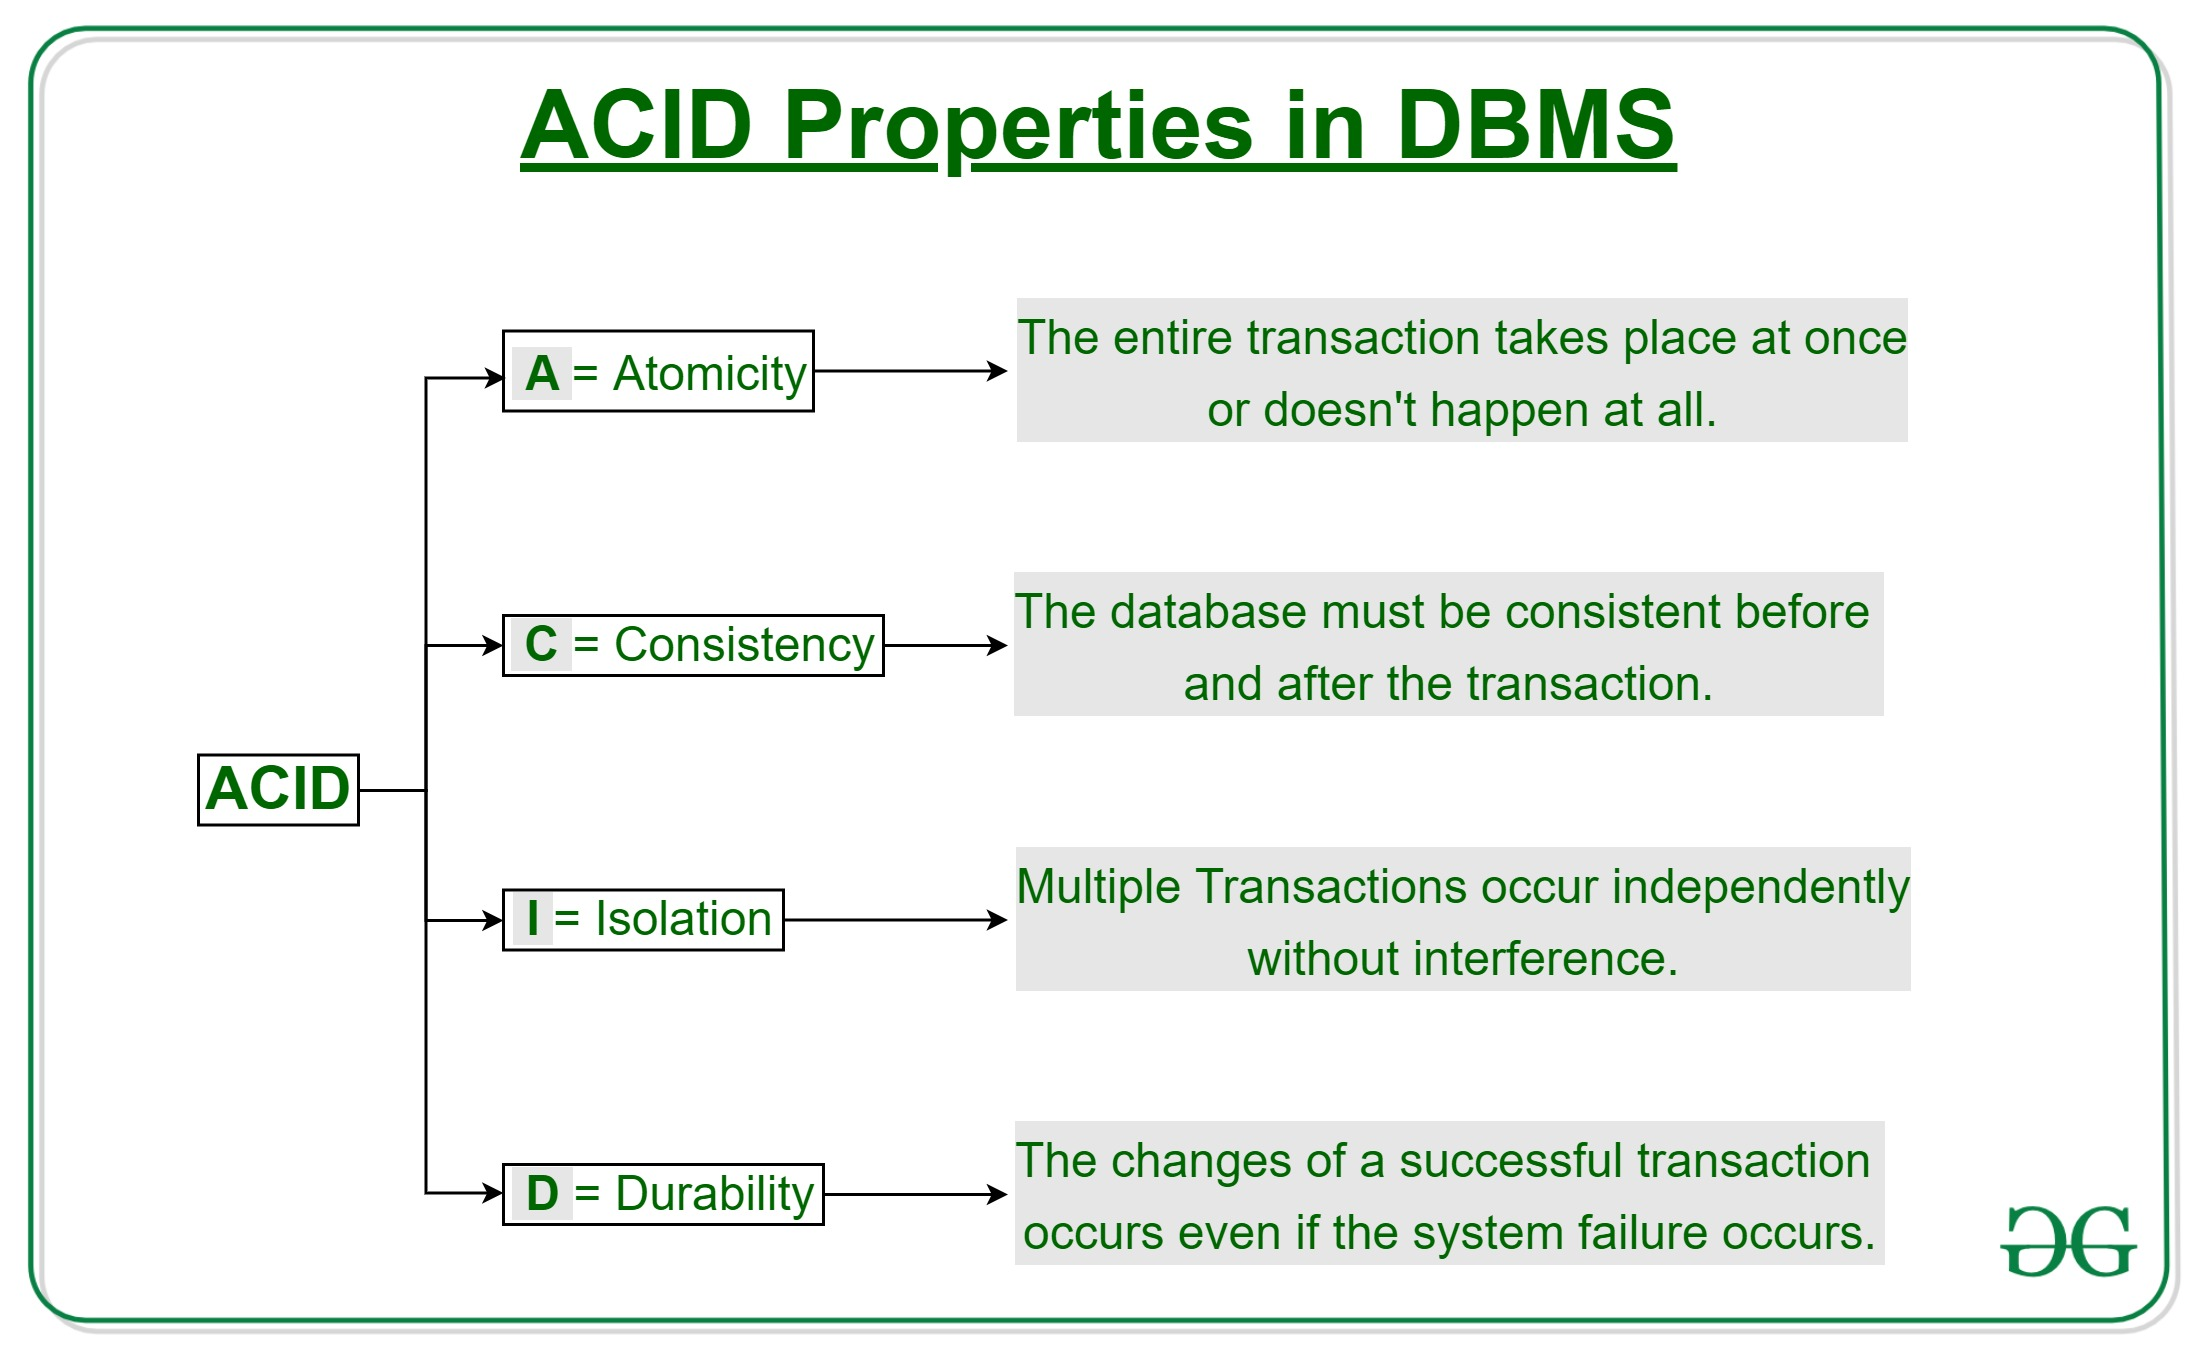
\includegraphics[scale=0.15]{images/ACID-Properties.jpg}
    \caption{ACID tulajdonságok}
    \label{fig:acid}
\end{figure}

Tehát csak olyan adatbázisok jöhetnek szóba a program implementálásánál aminek az integritása garantálható.
Hogy 2 eltérő adatbázist hasonlítsunk össze, egy SQL és egy NoSQL adatbázis ami teljesíti az ACID integritást megfelelő lesz.
A PostgreSQL adatbázis kíváló relációs adatbázis, nem véletlen, hogy az egyik legelterjedtebb. Teljesíti az ACID tulajdonságokat, és már 35 éve használják így biztosan megfelelően tesztelt.
A MongoDB dokumentum alapú adatbázis ACID, de csak dokumentum szintent. A mi szimulációnkhoz viszont így is megfelel a követelményeknek.
Érdekességként, a legtöbb dokumentum alapú adatbázis nem ACID, ezért nem annyira népszerűek.

\subsection{Protokollok és adatbázisok szerepe a programban}
A drón raj programot és az adatközpontot úgy tervezzük meg, hogy a telemetria adatok küldéséhez használt rész kicserélhető legyen valamilyen módon (például dependency injekción keresztül).
Így valósítjuk meg a több protokollon keresztüli kommunikációt. Az adatbázis végpontot is hasonlóan ki kell tudnunk cserélni, hogy ne kelljen módosítani a programon a különböző szimulációkhoz.
A következő kód példában láthatjuk, hogy működhet a dependency injekció. Itt a postgreSQL adatbázissal hoztuk létre a szervízt, de a mongoDB adatbázissal is létrehozhatjuk, ha teljesíti az interfész követelményeit.
\begin{python}
    postgresStorage, err := postgres.NewStorage(config.PostgresConfig)
    if err != nil {
        log.Println("Error connecting to database")
        panic(err)
    }
    mongoStorage, err := mongodb.NewStorage(config.MongoConfig)
    if err != nil {
        log.Println("Error connecting to database")
        panic(err)
    }
    var ts telemetry.Service
    var ds drone.Service
    var rs routing.Service
    ts = telemetry.NewService(postgresStorage, logger)
    rs = routing.NewService(logger)
    ds = drone.NewService(postgresStorage, jsonAdapter, logger, rs)
\end{python}

%TODO: ide még írni és a program struktúráját jobban megmutatni, a konkrét jegyzék struktúra is akár, hogy mi tartozik infrastruktúrához, mi a program magja stb. Interfacek kapcsolata,
%TODO: Új section ami a program folyamatával foglalkozik, nem a struktúrával
\Section{Szimuláció működésének folyamata}

A szimuláció működése azzal kezdődik, hogy elindítjuk az adatközpont programot.
Felcsatlakozik az adatbázisokra, majd létrehozza a szervizeket, és a REST API-n várja a bejövő kéréseket.
Ez lehet például egy konfigurációs kérés, a drónok lekérdezése, vagy a szállítás indítása.

Közben a drón-raj program is elindul, ez a program is egy REST API-n várja a kéréseket.
A drón raj program az API-n megkapja a drónokat és a hozzájuk rendelt csomagokat, majd megkezdódik a szimuláció, a drón-raj program telemetria adatokat küld az adatközpont programnak.
A drón-raj program olyan telemetria adatokat fog generálni, amelyek minél jobban a valsóságot tükrözik és ezeket az adatokat tovább fogja küldeni az adatközpontnak.
\begin{python}
{
    "telemetry": {
    "speed": 2,
    "location": {
    "latitude": 48.08092020178216,
    "longitude": 20.766208061642047
    },
    "altitude": 50,
    "bearing": 178.68412647009515,
    "acceleration": 0,
    "battery_level": 98,
    "motor_temperatures": [
    41,
    43
    ],
    "time_stamp": "2021-04-01T15:04:05.630Z",
    "drone_id": 2
    }
}
\end{python}

Ezeket a telemetria adatokat az adatközpont program fogadja a megadott porton és és lementi az adott adatbázisba. \ref{fig:adatkozpont-flow}

\begin{figure}[h]
    \centering
    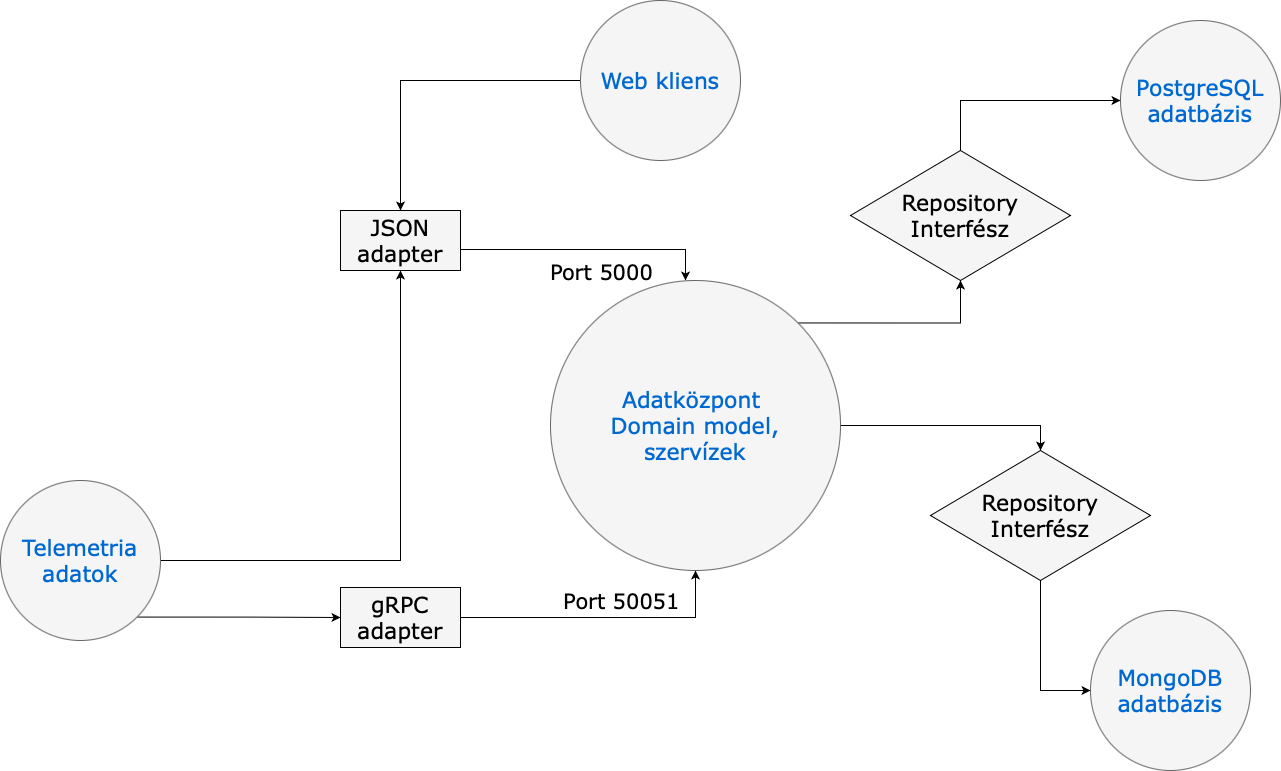
\includegraphics[scale=0.3]{images/adatkozpont-flow.png}
    \caption{Adatközpont program működésének folyamata}
    \label{fig:adatkozpont-flow}
\end{figure}


\Section{Táblázatok}

Táblázatokhoz a \texttt{table} környezetet ajánlott használni.
Erre egy minta \aref{tab:minta} táblázat.
A hivatkozáshoz az egyedi \texttt{label} értéke konvenció szerint \texttt{tab:} prefixszel kezdődik.

\begin{table}[h]
\centering
\caption{Minta táblázat. A táblázat felirata a táblázat felett kell legyen!}
\label{tab:minta}
\begin{tabular}{l|c|c|}
a & b & c \\
\hline
1 & 2 & 3 \\
4 & 5 & 6 \\
\hline
\end{tabular}
\end{table}

\Section{Ábrák}

Ábrákat a \texttt{figure} környezettel lehet használni.
A használatára egy példa \aref{fig:cimer}. ábrán látható.
Az \texttt{includegraphics} parancsba 
Az ábrák felirata az ábra alatt kell legyen.
Az ábrák hivatkozásához használt nevet konvenció szerint \texttt{fig:}-el célszerű kezdeni.

\begin{figure}[h]
\centering

\includegraphics[scale=0.3]{images/me_logo.png}
\caption{A Miskolci Egyetem címere.}
\label{fig:cimer}
\end{figure}

\Section{További környezetek}

A matematikai témájú dolgozatokban szükség lehet tételek és bizonyításaik megadására.
Ehhez szintén vannak készen elérhető környezetek.

\begin{definition}
Ez egy definíció
\end{definition}

\begin{lemma}
Ez egy lemma
\end{lemma}

\begin{theorem}
Ez egy tétel
\end{theorem}

\begin{proof}
Ez egy bizonyítás
\end{proof}

\begin{corollary}
Ez egy tétel
\end{corollary}

\begin{remark}
Ez egy megjegyzés
\end{remark}

\begin{example}
Ez egy példa
\end{example}

